\section{Relative positioning}

A relative position is a position that is relative to something absolute. A technique called dead reckoning is very useful in situations where one have to move away from a absolute position, therefore will not be able to get another for a while. Such as in a network game or outside hiking with no Global Positioning System (GPS). To use dead reckoning you need to keep track of things that can help you navigate, such as:

\begin{itemize}
\item Direction of travel.
\item Pace.
\item Time of walking.
\item Landmarks.
\end{itemize}

When our hiking trip starts, we know we are at a absolute position, that is our base camp, and we want to reach the destination as shown in figure \ref{fig:deadrecdrawing}. We use our pace, compass and the landmarks to navigate to the destination.

\begin{figure}[H]
	\centering
	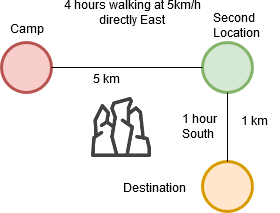
\includegraphics[width=0.4\linewidth]{positioning/positioning/deadRecDrawing}
	\caption{A hiking trip with navigation using dead reckoning.}
	\label{fig:deadrecdrawing}
\end{figure}

But dead reckoning suffers from errors that are cumulative, for example, if the first part of the trip had ended up being 8 kilometers instead of 5 then even if the second part goes according to plan, you are still going to end up in the wrong place. A way to solve this problem is to find your absolute location with bearings from time to time as that will reset the drift in regard to possible errors.

\section{Dead recking in network games}

Dead recking is not only used at sea or to navigate at land, but also in distributed virtual environments. When people across the planet play network games, they are sometimes located very far from each other, geographically. Pantel and Wolf\footnote{\cite{Pantel2002}} explores different dead reckoning schemes in various games such as sports and action games. They measured eight prediction schemes: Four predictions of positions, three predictions of input and one with no prediction. As shown in Figure \ref{fig:wolfpeperimage} Prediction 1 which predicts the position by assuming a constant velocity yields the best result.

\begin{figure}[H]
	\centering
	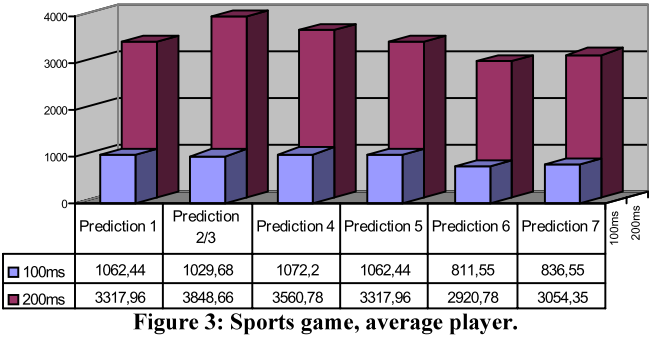
\includegraphics[width=0.5\linewidth]{positioning/positioning/wolfpeperImage}
	\caption{Prediction 1 was best in a sports game}
	\label{fig:wolfpeperimage}
\end{figure}

The article concludes that the different schemes tested upon were useful for network games, but could not reduce the latency directly, the impact, on the game, could be reduced however.